\documentclass[a4paper,10pt,twoside]{article}
%\usepackage{amssymb}
%\usepackage{amsthm}
\usepackage[polish]{babel}
\usepackage[utf8]{inputenc}
\usepackage[T1]{fontenc}
\usepackage{indentfirst}
\usepackage{caption}
\usepackage[top=2.5cm, bottom=2.5cm, left=2.5cm, right=2.5cm]{geometry}
\usepackage{graphicx}
\usepackage{amsmath}
\usepackage{booktabs}

\begin{document}
	
	\begin{center}
		\bgroup
		\def\arraystretch{1.5}
		\begin{tabular}{|c|c|c|c|c|c|}
			\hline
			EAIiIB & \multicolumn{2}{|c|}{Michał Kilian} & Rok II & \multicolumn{2}{|c|}{Grupa 5a} \\
			\hline
			\multicolumn{3}{|c|}{\begin{tabular}{c}Temat: \\ Wahadło proste \end{tabular}} & 
			\multicolumn{3}{|c|}{\begin{tabular}{c}Numer ćwiczenia: \\ 0 \end{tabular}} \\
			\hline
			\begin{tabular}{@{}c@{}}Data wykonania\\10.10.2018r.\end{tabular} & \begin{tabular}{@{}c@{}}Data oddania\\12.10.2018r.\end{tabular} & 
			\begin{tabular}{c}Zwrot do\\poprawki\\\phantom{data} \end{tabular} & \begin{tabular}{c}Data oddania\\\phantom{data}\end{tabular} &
			\begin{tabular}{@{}c@{}}Data zaliczenia\\\phantom{data}\end{tabular} & \begin{tabular}{c}Ocena\\\phantom{ocena}\end{tabular} \\[4ex]
			\hline
		\end{tabular}
		\egroup
	\end{center}
	
	\section{Cel ćwiczenia}
	Zaznajomienie się
	z typowymi metodami opracowania danych pomiarowych
	przy wykorzystaniu wyników pomiarów dla wahadła pro
	stego 
	

	Wahadło matematyczne to punktowa masa $m$ zawieszona na nieważkiej i nierozciągliwej lince poruszająca w jednorodnym polu grawitacyjnym.
	W doświadczeniu wykorzystamy bardzo dobre przybliżenie takiego układu jakim jest ciężka metalowa kulka zawieszona na nitce.
	
	Aby znacząco uprościć obliczenia przyjmiemy $\sin\theta\approx\theta$ co jest prawdą dla małych wartości kąta $\theta$ zgodnie z
	twierdzeniem Taylora. Dzięki temu ograniczamy wpływ oporu powietza na wyniki, a z uproszczonego równania ruchu wahadła
	uzyskujemy następujacą zależność
	\begin{equation}
	T=2\pi\sqrt{\frac{l}{g}}
	\end{equation}
	gdzie $T$ - okres drgań, $l$ - długość nici, $g$ - przyspieszenie grawitacyjne. Po przekształceniu otrzymujemy wzór roboczy pozwalający
	na wyznaczenie wartości przyspieszenia grawitacyjnego dla Ziemi
	\begin{equation}
	\label{eq:working_g}
	g=\frac{4\pi^2l}{T^2}
	\end{equation}
	
	\section{Opis doświadczenia}
	

	Ćwiczenie składa się z 2 części, w pierwszej dokonujemy pomiarów dla ustalonej długości wahadła, a w drugiej wyznaczamy
	przyspieszenie grawitacyjne $g$ za pomocą regresji liniowej.
	
	\begin{figure}[!htp]
		\centerline{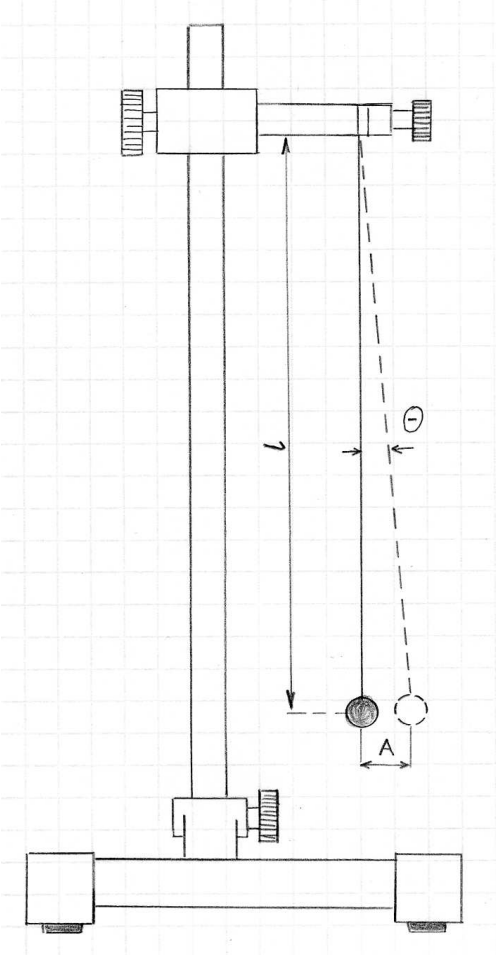
\includegraphics[scale=0.18]{wahadlo}}
		\caption{Zestaw użyty w doświadczeniu}
	\end{figure}
	
	
	Na statywie zawieszono metalową kulkę na nici. Przed rozpoczęciem doświadczenia została zmierzona długość powstałego w ten sposób
	wahadła za pomocą linijki. Następnie zmierzono stoperem czas trwania 20 okresów drgań wahadła. Wyniki umieszczono w tabeli.
	
	\newpage
	\section{Wyniki pomiarów}
	
	\begin{table}[!htbp]
		\caption{Pomiar okresu drgań przy ustalonej długości wahadła\newline
			 długość wahadła \hspace{60pt}$l=50,1cm$\newline
		 niepewność pomiaru  \hspace{40pt} $u(l) = 0,1cm$}
		\centering
		\def\arraystretch{1.4}
		\begin{tabular}{|c|c|c|c|}
			\hline
			Lp. & liczba okresów \textit{k} &  czas \textit{t} dla \textit{k} okresów [s] & Okres $T_i = t/k$[s] \\ \hline
			1 & 20 & 28.45 & 1,4225 \\ \hline
			2 & 20 & 28.5 & 1,425 \\ \hline
			3 & 20 & 28,37 & 1,4185 \\ \hline
			4 & 20 & 28,21 & 1,4105 \\ \hline
			5 & 20 & 28,29 & 1,4145\\ \hline
			6 & 20 & 28,56 & 1,428\\ \hline
			7 & 20 & 28,48 & 1,424\\ \hline
			8 & 20 & 28,52 & 1,426\\ \hline
			9 & 20 & 28,47 & 1,4235 \\ \hline
			10 & 20 & 28,39 & 1,4195\\ \hline
		
		\end{tabular}
	\end{table}
	
	\begin{table}[!htbp]
		\caption{Pomiar zależności okresu drgań od długości wahadła}
		\centering
		\def\arraystretch{1.4}
		\begin{tabular}{|c|c|c|c|c|c|}
			\hline
			Lp. & \textit{l} [mm] & \textit{k} & \textit{t} [s] & $ T_i$ [s] & $T_i^2$[$s^2$] \\ \hline
			1 &501& 20 & 28.424 & 1,4212 & 2,0198\\ \hline
			2 &475& 20 & 27,626 & 1,3825 & 1,9080\\ \hline
			3 &450& 20 & 27,160 & 1,3456 & 1,8442\\ \hline
			4 &431& 20 & 26,096& 1,3169 & 1,7025\\ \hline
			5 &402& 20 & 25,626& 1,2719 & 1,6417\\ \hline
			6 &352& 20 & 24,002 & 1,1901 & 1,4402\\ \hline
			7 &302& 20 & 21,974 & 1,1024 &1,2071\\ \hline
			8 &281& 20 & 21,184 & 1,0634 & 1,1219\\ \hline
			9 &250& 20 & 20,002 & 1,0030 & 1,002\\ \hline
			10 &219& 20 & 18,768 & 0,9387 &0,8806\\ \hline
			11 &198& 20 & 18,204 & 0,8926 &0,8285\\ \hline
			12 &178& 20 & 16,826 & 0,8463 &0,7078\\ \hline
			13 &150& 20 & 15,184 & 0,7769 &0,5764\\ \hline
			14 &120& 20 & 13,938 & 0,6949 &0,4857\\ \hline
			15 &101& 20 & 12,712 & 0,6375 &0,4040\\ \hline
		\end{tabular}
	\end{table}
	
	\section{Opracowanie wyników}
	\noindent
	
	\paragraph{Ocena błęów grubych} Wszystkie wyniki wynoszą nieco ponad 28 sekund i żaden nie odstaje znacząco od reszty co pozwala założyć, że nie popełniliśmy żadnego błędu grubego podczas pomiarów
	
	\paragraph{Ocena niepewności pomiaru (typu A)} obliczam $\bar{x}$ ze wzoru $\bar{x} = \frac{1}{n} \sum x_i$ \\
	$T_0 = \frac{(1,4225s +	1,425s +	1,4185s +
	1,4105s + 
	1,4145s +
	1,428s +
	1,424s +
	1,426s +
	1,4235s + 
	1,4195s)}{10} = 1,4212s
	$ \\
	ze wzoru $u(x) \equiv s_x = \sqrt{\frac{\sum(x_i - \bar{x})^2}{n(n-1)}}$ liczę niepewność pomiaru okresu (typu A)\\ $u(T_0) = \sqrt{\frac{(1,4225s-1,4212s)^2 + (1,425s- 1,4212s)^2 + ... +(1,4195s-1,4212s)^2 +}{9*10}} = 0,017s $
	\paragraph{Ocena niepewności pomiaru długości wahadła (typu B)} Niepewność pomiaru długości wahadła (typu B) jest równa działce elementarnej użytego przyrządu. W tym przypadku użyto miarki więc $u(l) = 1mm$ 
	\\
	\paragraph{Obliczenie przyspieszenia ziemskiego} Przekształcamy wzór $T = 2\pi\sqrt{\frac{l}{g}} $ do postaci $g = \frac {4*\pi^2l}{T^2}$ po podstawieniu $g = \frac {4*\pi^2*0,501m}{(1,4212s)^2} = 9,7923\frac{m}{s^2}$
	\\
	\paragraph{Obliczenie niepewności złożonej}
	Obliczamy niepewności z prawa przenoszenia niepewności \\$\frac{u_c(y)}{y} = \sqrt{\sum_{k}[p_k\frac{u(x_k)}{x_k}]^2}$
	\\ W naszym przypadku $\frac{u_c(y)}{y} = \sqrt{\left(\frac{u(l)}{l}\right)^2 + \left(\frac{-2*u(T)}{T}\right)^2} $
	  $	\frac{u(g)}{g} = \sqrt{\left(\frac{1mm}{501mm}\right)^2 + \left(\frac{-2*0,0017s}{1,4212s}\right)^2} = 0,3\%$
	  \\Niepewność bezwględna $u_c(g) = 9,7924 \frac{m}{s^2} * \frac{0,3\%}{100\%} = 0,029\frac{m}{s^2}$
	  \\
	  \paragraph{Obliczenie niepewności rozszerzonej} Obliczamy niepewność rozszerzoną ze wzoru $U(g) = ku(g)$ przyjmując k = 2 $U(g) = 2*0,029 \frac{m}{s^2} = 0,058 \frac{m}{s^2}$
	  \\
	  \paragraph{Porównanie z wartością tabelaraczyną}  Różnica w stosunku do wartości tabelarycznej dla Krakowa wynosi $9,811 \frac{m}{s^2} - 9,792 \frac{m}{s^2} = 0,019  \frac{m}{s^2}$ co jest mniejsze niż nasza niepewność rozszerzona więc można uznać, że zmierzone przyspieszenie jest zgodne z wartością tabelaryczną 
	
	\begin{figure}[h]
		\centering{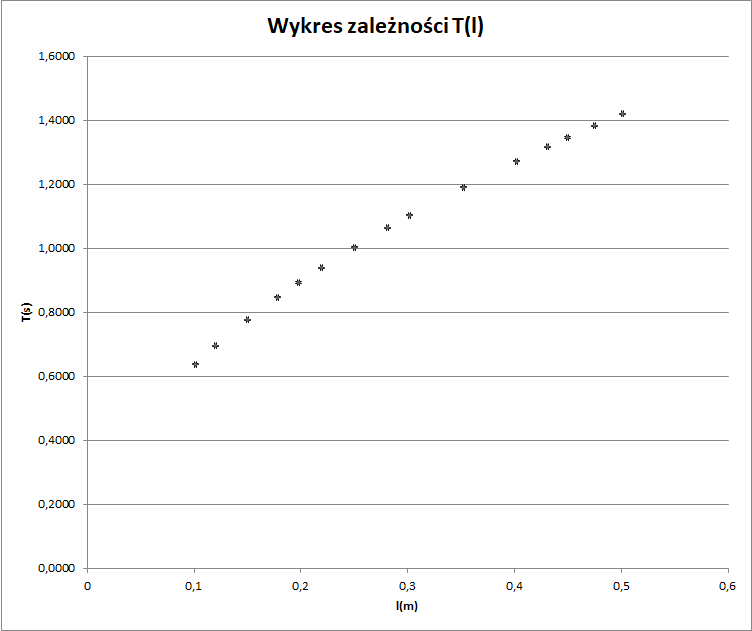
\includegraphics[scale=0.6]{w2}}
		\caption{Wykres powstały z pomiarów okresu dla różnych długości nici}
	\end{figure}
	
	\begin{figure}[h]
		\centering{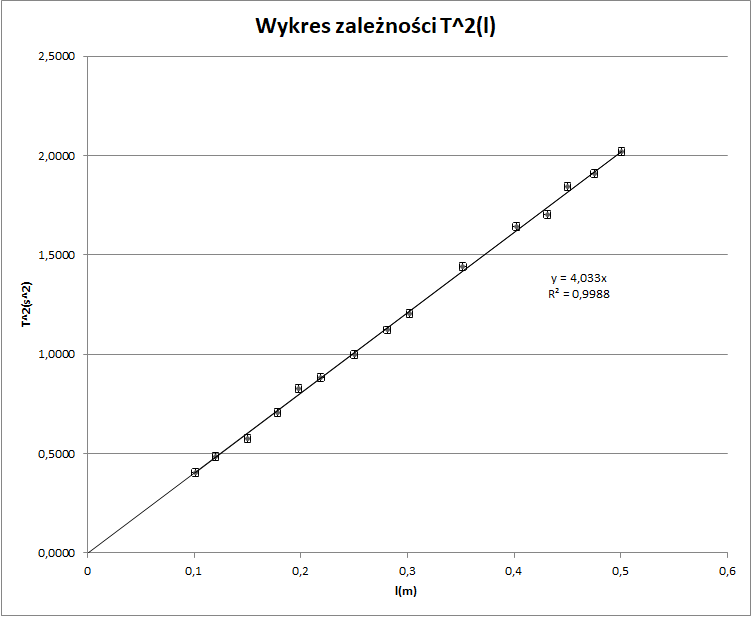
\includegraphics[scale=0.8]{w1}}
		\caption{Wykres zlinearyzowany $T^2$
						w funkcji 
			$l$ wraz z dopasowaną prostą}
	\end{figure}
	
	\paragraph{Obliczenie wartości g z współczynnika nachylenia } Oczytujemy współczynnik nachylenia z wykresu $a  = 4,033$ Korzystamy ze wzoru $a = \frac{4\pi^2}{g}$ \\ $g = \frac{4\pi^2}{a} = \frac{4\pi^2}{4,033} = 9,7889 \frac{m}{s^2}$
	
	\paragraph{Obliczenie niepewności u(g) na podstawie niepewności u(a)}
	Niepewność $u(a)$ odczytujemy z wyniku działania funkcji excel $u(a) = $ Korzystamy z prawa przenoszenia niepewności $\frac{u_c(y)}{y} = 0,0024 \sqrt{\sum_{k}[p_k\frac{u(x_k)}{x_k}]^2}$ \\ W naszym przypadku $$\frac{u_c(g)}{g} = \sqrt{[p_k\frac{u(a)}{a}]^2} = \sqrt{[\frac{-1 * 0,0024 }{4,033}]^2} = \frac{0,0024}{4,033} = 0,58\%$$ \\
	$u(g) = 9,7889\frac{m}{s^2} * 0,58\% = 0,0058\frac{m}{s^2}$ %dopisać
	\section{Wnioski}
	Wahadło matematyczne pozwala w dość prosty sposób wyznaczyć przybliżoną wartość przyspieszenia grawitacyjnego. Uzyskane wyniki, zarówno bezpośrednio z pomiarów jak i korzystając z współczynnika nachylenia prostej dopasowanej do wykrsu są bliskie wartości tabelarycznej. Błędy mogą być spowodowane faktem, że nitka nie była nieważka. Ciało natomiast miało swoje rozmiary, a nie było punktem materialnym czego wymaga wahadło matematyczne.
\end{document}
















\end{}